\documentclass[a4paper, 12pt]{article}
\usepackage[T2A,T1]{fontenc}
\usepackage[utf8]{inputenc}
\usepackage[english, russian]{babel}
\usepackage{graphicx}
\usepackage[hcentering, bindingoffset = 10mm, right = 15 mm, left = 15 mm, top=20mm, bottom = 20 mm]{geometry}
\usepackage{multirow}
\usepackage{lipsum}
\usepackage{amsmath, amstext}
\usepackage{siunitx}
%\usepackage{subcaption}
\usepackage{wrapfig}
\usepackage{mathrsfs}
\usepackage{adjustbox}
\usepackage{enumerate, indentfirst, float}
\usepackage{pgffor}
\usepackage{capt-of, svg}
\usepackage{array}
\usepackage{longtable}
\usepackage{csvsimple}
\usepackage{pdfpages}
\usepackage{subfigure}
\usepackage{sectsty}

\newenvironment{bottompar}{\par\vspace*{\fill}}{\clearpage}
 
\sectionfont{\fontsize{12}{18}\selectfont}

\begin{document}
\begin{titlepage}

\newcommand{\HRule}{\rule{\linewidth}{0.5mm}} % Defines a new command for the horizontal lines, change thickness here

\center % Center everything on the page
 
%----------------------------------------------------------------------------------------
%	HEADING SECTIONS
%----------------------------------------------------------------------------------------

\textbf{\LARGE Московский Физико-Технический}
\\[5pt]
\textbf{\LARGE Институт}\\[1,5cm] % Name of your university/college
\textsc{\Large кафедра общей физики}\\[0.5cm] % Major heading such as course name
\textsc{\large Лабораторная работа  4.3.5}\\[0.9cm] % Minor heading such as course title

%----------------------------------------------------------------------------------------
%	TITLE SECTION
%----------------------------------------------------------------------------------------



{ \huge \bfseries Изучение голограммы}
\\[1.7cm] % Title of your document




 
%----------------------------------------------------------------------------------------
%	AUTHOR SECTION
%----------------------------------------------------------------------------------------

\begin{minipage}{0.3\textwidth}
	\begin{flushleft} \large
		\emph{Студент:}\\
		\textbf{Шиянов Кирилл}% Your name
	\end{flushleft}
\end{minipage}
~
\begin{minipage}{0.5\textwidth}
	\begin{flushright} \large
		\emph{Преподаватель:} \\
		\textbf{Фёдоров Георгий Евгеньевич} % Supervisor's Name
	\end{flushright}
\end{minipage}

\begin{bottompar}
	
	{\large \today}

\end{bottompar}
\vfill % Fill the rest of the page with whitespace

\end{titlepage}

\section*{Цель работы:}

\noindent изучить свойства голограмм точечного источника и объёмного предмета.

\section*{В работе используются: }
\begin{itemize}
\item гелий-неоновый лазер; 
\item голограммы; 
\item набор линз; 
\item предметная шкала;
\item экран;
\item линейка.
\end{itemize}	

\section*{Рабочие формулы}  




\noindent Формула для дифракции Фраунгофера:
\begin{equation}
\frac{\lambda}{D }= \frac{\Delta x}{L}
\end{equation}
\noindent где $\Delta x$ - расстояние между дифракционными максимумами на экране, L -  расстояние от шкалы до экрана, D - цена деления шкалы.
\\
\\
\noindent Формула тонкой линзы:
\begin{equation}
\frac{1}{F} = \frac{1}{a} +  \frac{1}{b}
\end{equation}
\noindent где F - фокусное расстояние, a - расстояние до источника, b - расстояние до изображения.
\\
\\
\noindent Для радиусов колец голограммы точечного источника:
\begin{equation}
R = \sqrt{m\lambda d}
\end{equation}
\noindent где $m$ - номер кольца, $d$ - расстояние от точечного источника до фотопластинки (или голограммы)

\section*{Оптическая схема}

\begin{figure}[H]
	\centering
	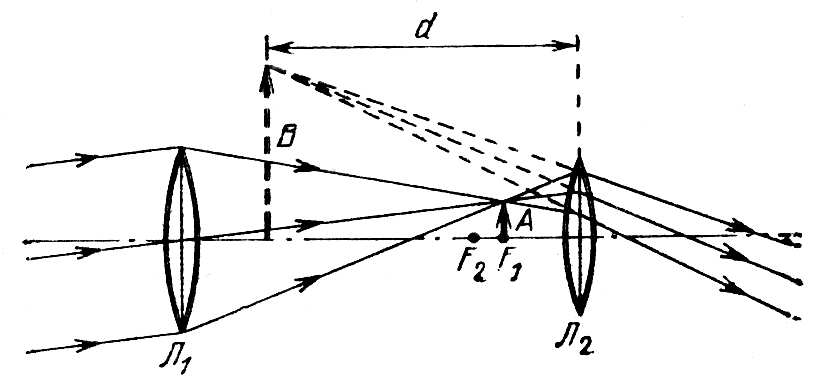
\includegraphics[width = 17 cm]{1.png}
	\caption{Схема установки: Г - голограмма}
\end{figure}



\section*{Ход работы}
\section{Определение цены деления}
\noindent Включим лазер и определим цену деления предметной шкалы. Установим кассету с транспарантами вблизи лазера. Осветим шкалу и получим четкую дифракционную картину. 

\noindent Цену деления рассчитаем по формуле для дифракции Фраунгофера: 
\[ D = \dfrac{L\lambda}{\Delta x}, \] 
\noindent где $\Delta x$~--~расстояние между дифракционными максимумами, $L$~--~расстояние от шкалы от экрана.
\[\Delta x = (5.0\pm 0.1) \; mm, \quad L = (120\pm2) \; cm, \quad \lambda = 532 \; nm, \]
\noindent тогда $D = (1.28 \pm 0.06) \cdot 10^{-4} \; m$~--~цена деления предметной шкалы.

\noindent Определим цену деления вторым методом, установив линзу с фокусным расстоянием $F\approx4 \;cm$ и получим в центре экрана увеличенное изображение предметной шкалы с четкими делениями.

\noindent Измерим расстояния от линзы до предметной шкалы $a$ и до экрана $b$ и рассчитаем увеличение системы. Определите расстояние $D$ между изображениями штрихов и рассчитаем цену деления D предметной шкалы:
\[\Delta x = \frac{(51.0\pm0.5)\; mm}{20} = (2.55\pm0.03) \; mm , \quad a = (58\pm1) \; mm, \quad b = (1055\pm1) \; mm, \]
\[D = \dfrac{a\Delta x}{b} = (1.4 \pm 0.05) \cdot 10^{-4} \; m \]

\newpage


\section{Точечный источник}

\noindent Получаем на экране изображение голограммы точечного источника -- наиболее четкое изображение колец. Сфотографируем кольца на фоне линейки (см. Приложение 1). Обработаем полученное изоброжение с помощью ImageJ: найдём минимумы интенсивности вдоль радиальной прямой. С учётом масштаба 0.0496 pxl/mm найдём значения для радиусов колец в mm. Затем, зная увеличение системы $\Gamma = \frac{995\; mm}{58 \; mm} = 17$, расчитаем радиусы колец голограммы.



\begin{table}[H]
	\centering
	\begin{tabular}{|c|c|c|c|c|c|}
		\hline

m&x, pxl&R, pxl&R, mm&r, mm&$r^2, mm^2$\\ \hline
0&981&0&0.0&0.00&0.00\\ \hline
1&1026&45&2.2&0.13&0.02\\ \hline
2&1048&67&3.3&0.19&0.04\\ \hline
3&1065&85&4.2&0.24&0.06\\ \hline
4&1081&100&5.0&0.29&0.08\\ \hline
5&1090&109&5.4&0.32&0.10\\ \hline
6&1102&121&6.0&0.35&0.12\\ \hline
7&1116&135&6.7&0.39&0.15\\ \hline
8&1127&146&7.2&0.42&0.18\\ \hline
9&1135&154&7.6&0.45&0.20\\ \hline
10&1142&161&8.0&0.47&0.22\\ \hline
11&1151&170&8.4&0.49&0.24\\ \hline
12&1158&178&8.8&0.51&0.26\\ \hline
13&1167&186&9.2&0.54&0.29\\ \hline
14&1174&194&9.6&0.56&0.31\\ \hline
15&1182&201&10.0&0.58&0.34\\ \hline
16&1189&208&10.3&0.60&0.36\\ \hline
17&1194&213&10.6&0.62&0.38\\ \hline
18&1201&220&10.9&0.64&0.41\\ \hline
19&1206&226&11.2&0.65&0.43\\ \hline
20&1211&230&11.4&0.67&0.44\\ \hline
21&1219&238&11.8&0.69&0.47\\ \hline
22&1227&246&12.2&0.71&0.51\\ \hline
23&1231&250&12.4&0.72&0.52\\ \hline
24&1236&255&12.6&0.74&0.54\\ \hline
25&1241&260&12.9&0.75&0.57\\ \hline
26&1245&264&13.1&0.76&0.58\\ \hline
\end{tabular}
\caption{Радиусы темных колец и расстояния до источника при создании голограммы}
\end{table}

\begin{figure}[H]
	\centering
	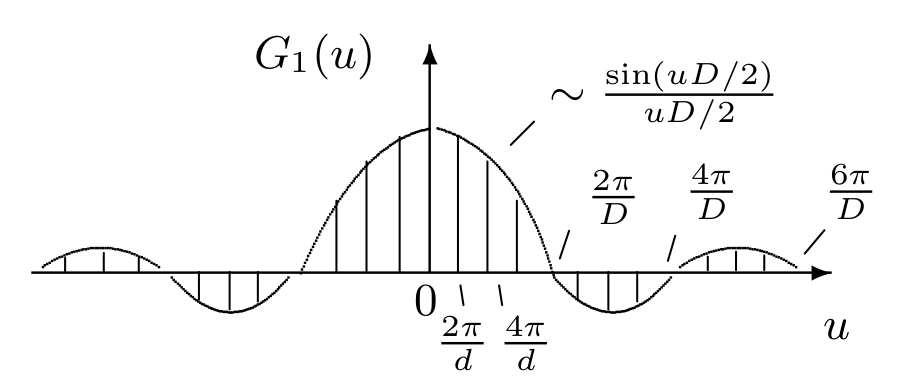
\includegraphics[width = 16 cm]{2.png}
	\caption{Квадрат радиуса кольца от его номера}
\end{figure}


\noindent Из (3) расстояние от источника, который был использован при её создании, до голограммы: 
\[ d_1 = \frac{1}{\lambda}\frac{\Delta (r^2)}{\Delta m}\]
\[\frac{\Delta (r^2)}{\Delta m} = (2.29 \pm 0.05) \cdot 10^{-2}\; mm^2 \]
\[d_1 = (43 \pm 1) \;mm \]

\noindent Перемещая линзу вдоль луча, получаем на экране изображение сначала мнимого $O_2$, затем действительного источника $O_3$.
Измерив расстояния $b_i$ от линзы до изображений, посчитаем расстояния $a_i = \frac{Fb_i}{b_i - F}$ от точечных источников до линзы. Зная расстояние $s_i$ между линзой и голограммой находим расстояния $d_i = |s_i-a_i|$ от точечных источников до голограммы:

\[b_2 = 1055 \; mm\]
\[b_3 = 970 \;  mm\]
\[s_2 = 4 \; mm\]
\[s_3 = 78 \;  mm\]

\noindent Тогда:

\[a_2 = 41.6 \; mm\]
\[a_3 = 41.7 \;  mm\]

\[d_2 = 38 \; mm\]
\[d_3 = 36 \; mm\]

\newpage
\section{Изучение фокусирующих свойств голограммы}

\noindent Добиваемся полного разделения пучков света на экране и определяем, какой из них соответствует действительному, какой мнимому изображению. 

\noindent Установив перед голограммой предметную шкалу, получаем четкое изображение шкалы в пятне, соответствующем действительному изображению.

\noindent Измерьте расстояние между штрихами $ \Delta x $ на экране и расстояние $L$ от экрана до голограммы. Используя эти данные, а также найденную ранее цену деления шкалы $D$, рассчитаем фокусное расстояние голографической линзы.

\[ \Delta x = \frac{(9.5 \pm 0.5) \; mm}{7} = (1.36\pm 0.07) \; mm   ; \quad L = (510 \pm 5) \; mm \]
\[ F = \dfrac{L}{1+\frac{D}{\Delta x}} = (4.6 \pm 0.1) \; cm \]

\section{Изучение характеристик голограммы объемного предмета}
\subsection{Изучение мнимого изображения}

\noindent Настроив систему и поместив голограмму в расширенный пучок лазера фотоэмульсией к лазеру находим мнимое изображение предмета. 
$ \alpha = 32^o \pm 2^o $~--~угол поворота голограммы (угол падения опорного пучка).

\noindent Постепенно закрываем голограмму листом бумаги и видим, что изображение почти не меняется, то есть восстанавливается не из полной картины.

\noindent На мнимом изображении видим линейку, а за ней стержень. На действительном изображении стержень расположен перед линейкой. 

\noindent Оценим расстояние $h$ от линейки до вертикального стержня. Для этого рассмотрим отметку на линейке при разных углах поворота. Для угла $\alpha = 30^o$ при повороте на $\Delta \alpha =  10^o$ стержень соответствует делениям отстоящим на $l = 6$ мм. Тогда: \[h \approx \frac{l \cos \alpha}{\Delta \alpha} = 3 \; cm \]


\subsection{Изучение действительного изображения}

\noindent Находим действительное изображение, поворачиваем голограмму на $180^o$ вокруг вертикальной оси.

\noindent Угол падения восстанавливающей волны, при которых возникает действительное изображение~--~$30^o$, мнимое изображение~--~$24^o$.

\noindent Снова разворачиваем голограмму эмульсией к лазеру. Перемещаем короткофокусную линзу расширителя вдоль луча, наблюдаем, что при приближении линзы к лазеру изображение действительное увеличивается, мнимое уменьшается.


\section*{Вывод}  
	\noindent В данной работе мы определили характеристики голограммы точечного источника и исследовали голограмму трёхмерного объекта.


\section*{Приложение 1}  
\begin{figure}[H]
	\centering
	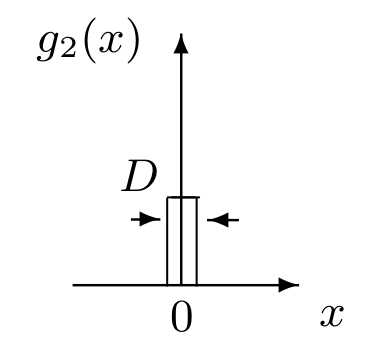
\includegraphics[width = 17 cm]{3.jpg}
	\caption{Изображение голограммы точечного источника}
\end{figure}

\end{document}